%%=============================================================================
%% Methodologie
%%=============================================================================

\chapter{\IfLanguageName{dutch}{Methodologie}{Methodology}}
\label{ch:methodologie}

%% TODO: Hoe ben je te werk gegaan? Verdeel je onderzoek in grote fasen, en
%% licht in elke fase toe welke stappen je gevolgd hebt. Verantwoord waarom je
%% op deze manier te werk gegaan bent. Je moet kunnen aantonen dat je de best
%% mogelijke manier toegepast hebt om een antwoord te vinden op de
%% onderzoeksvraag.

Om te kunnen onderzoeken hoe men een impressie zou kunnen wekken dat men met een echt persoon contact staat werd er gefocust op 2 belangrijke aspecten:

\begin{itemize}
    \item Welke narrow ai's dient men te combineren om bepaalde menselijke aspecten na te bootsten
    \item Belangrijkheid van deze aspecten bevragen
\end{itemize}

Eerst werd geschetst welke narrow ai's een mogelijke combinatie zouden kunnen zijn voor verschillende aspecten op vlak van beeld, spraak en kennis. Daarna werd aan de hand van een enquete getoetst welke aspecten het belangrijkste zijn voor de gebruiker, om deze ervaring te verkrijgen.

\newpage

\section{Menselijke aspecten}

Uiteraard is het schetsen van alle eigenschappen van een mens onbegonnen werk. Dit is bij elke persoon anders omdat iedereen andere karaktereigenschappen heeft. Ook zijn zaken zoals bijvoorbeeld een geweten of moraal één van de moeilijkste zaken om in een technologie te gieten. 

In dit onderzoek werd er op zoek gegaan naar de meest voor de hand liggende eigenschappen van een mens, niet bepaald het emotionele gegeven zoals bijvoorbeeld een geweten. Dit kan misschien wel een leuke uitbreiding zijn op deze bachelorproef voor een bachelorproef in het psychologie veld.

Om dit onderzoek te schetsen ging men er van uit dat men een ai zou willen opzetten die via bijvoorbeeld een videocall met video en spraak contact zou hebben met een persoon, en dat de tegenpartij niet kan onderscheiden of er contact gemaakt wordt met een technologie of een echte persoon.

Bovenstaande case werd opgesplitst in de drie meest voor de hand liggende delen:

\begin{itemize}
    \item Beeld
    \item Spraak
    \item Kennis
\end{itemize}

In de volgende subsecties werd dit meer in detail onderzocht

\newpage

\section{Beeld}

Op vlak van beeld werd er van uit gegaan dat onderstaande zaken het belangrijkste waren:

\begin{itemize}
    \item Gezichtsherkenning
    \item Emotieherkenning
    \item Deepfakes
\end{itemize}

Gezichtsherkenning: Een AI die in staat is om gezichten te herkennen en te onderscheiden. Dit kan helpen om gepersonaliseerde en aangepaste conversaties te bieden, bijvoorbeeld door de herkenning van emoties op het gezicht van de gesprekspartner.

Emotieherkenning: Het vermogen om emoties te herkennen via het gelaat en te interpreteren is essentieel voor effectieve communicatie tussen mensen. Een AI die menselijke emoties kan herkennen en daarop kan reageren, kan helpen om een meer natuurlijke conversatie te creëren.

Deepfakes: Door het gebruik van deepfakes, kan de AI gezichtsuitdrukkingen en andere non-verbale signalen nabootsen, waardoor de conversatie nog overtuigender wordt.

\newpage

\subsection{Gezichtsherkenning}

Gezichtsherkenning is een technologie die het mogelijk maakt om individuele gezichten te identificeren en te verifiëren op basis van specifieke kenmerken, zoals de afstand tussen de ogen, de neus en de mond, de vorm van het gezicht en de verhoudingen tussen deze kenmerken.

Er zijn verschillende methoden voor gezichtsherkenning, waaronder 2D-gezichtsherkenning, 3D-gezichtsherkenning en gezichtsherkenningsalgoritmen gebaseerd op artificiële intelligentie. 2D-gezichtsherkenning maakt gebruik van platte afbeeldingen van het gezicht om het te herkennen, terwijl 3D-gezichtsherkenning gebruik maakt van driedimensionale modellen van het gezicht om meer gedetailleerde en nauwkeurige identificatie te bieden.

Zoals hierboven besproken is dit interessant voor deze case om via deze manier gepersonaliseerde en aangepaste conversaties te bieden. Wanneer men focust op gezichtsherkenning gebaseerd op artificiële intelligentie dan komt men op  artificiële intelligentie die gebruik maakt van deep learning-technieken, waaronder convolutionele neurale netwerken (CNN's) en recurrente neurale netwerken (RNN's), om gezichten te herkennen en te identificeren.

\subsubsection{Onderzoek naar combinatie van Artificial Narrow Intelligences}

Wanneer men verschillende artificial narrow intelligences zou gaan willen combineren om gezichtsherkenning goed te laten verlopen denkt men in eerste instantie aan:

\begin{itemize}
    \item Computer vision
    \item Patroonherkenning
    \item Machine learning
\end{itemize}

In eerste instantie is het belangrijk dat dit onderdeel van de software in staat is om digitale beelden van gezichten te analyseren en verwerken. Via deze manier kan men belangrijke kenmerken van een gezicht, zoals bijvoorbeeld de ogen, neus en mond te identificeren. Dit is een onderdeel van computer vision.

Vervolgens zou men via patroonherkenning moeten kunnen herkennen welke combinaties van kenmerken bij een bepaald gezicht horen. Via deze gekende patronen kan men de identiteit van een persoon bepalen.

Bij zowel computer vision als patroonherkenning is machine learning een belangrijke tool om het gezichtsherkenningssysteem te verbeteren en te optimaliseren.

Zo kan machine learning bij computer vision worden gebruikt om het systeem te trainen om automatisch bepaalde kenmerken van een gezicht te herkennen, zoals de positie van de ogen, neus en mond. Hier kunnen convolutionele neurale netwerken voor worden gebruikt, die zeer handig zijn voor beeldverwerking.

Ook voor patroonherkenning kan machine learning worden gebruikt om het systeem te trainen om automatisch patronen in gezichtskenmerken te herkennen die uniek zijn voor een bepaald persoon.

\subsection{Emotieherkenning}

Emotieherkenning is het proces waarbij software of technologie wordt gebruikt om menselijke emoties te detecteren en te interpreteren op basis van gezichtsuitdrukkingen, stemintonatie en andere fysieke signalen.

Het maakt gebruik van verschillende methoden, waaronder beeld- en spraakverwerking, machine learning en artificiële intelligentie om emoties te identificeren en te classificeren. In het geval van emotieherkenning wordt gebruik gemaakt van computeralgoritmen om gezichtsuitdrukkingen te analyseren en te interpreteren, zoals glimlachen, fronsen en het bewegen van de wenkbrauwen.

Binnen emotieherkenning wordt artificiële intelligentie (AI) gebruikt om complexe patronen in de gegevens te ontdekken en te interpreteren. AI-algoritmen kunnen worden getraind om gezichtsuitdrukkingen te herkennen die specifiek zijn voor bepaalde emoties.

De meest gebruikte methode binnen AI voor emotieherkenning is machine learning. Hierbij worden de algoritmen getraind op een grote hoeveelheid gegevens om patronen te ontdekken en voorspellingen te doen over nieuwe gegevens. Het trainen van de algoritmen gebeurt meestal met behulp van datasets die handmatig zijn gelabeld door menselijke experts. Deze labels worden gebruikt om het algoritme te leren welke kenmerken overeenkomen met welke emoties.

Naast machine learning zijn er ook andere AI-technieken die worden gebruikt in emotieherkenning, zoals deep learning en neurale netwerken. Deze methoden maken gebruik van complexe wiskundige modellen die zijn ontworpen om grote hoeveelheden gegevens te verwerken en complexe patronen te identificeren.

\subsubsection{Onderzoek naar combinatie van Artificial Narrow Intelligences}

Wanneer men verschillende artificial narrow intelligences zou gaan willen combineren om emotieherkenning goed te laten verlopen denkt men in eerste instantie aan:

\begin{itemize}
    \item Computer vision
    \item Patroonherkenning
    \item Machine learning
\end{itemize}

De benodigde articial narrow intelligences die men dient te combineren zijn in eerste instantie dezelfde als bij gezichtsherkenning, omdat ze beide steunen op het visuele aspect.

Zo zal computer vision dienen om digitale beelden van gezichten te analyseren en verwerken om zo kenmerken in verband met gezichtsuitdrukkingen, zoals oog-, mond- en wenkbrauwpositie te identificeren.

Patroonherkenning zal dan op zijn beurt moeten kunnen herkennen welke patronen in gezichtsuitdrukkingen bij bepaalde emoties horen en deze patronen kunnen identificeren om op deze manier de emotie van een persoon te achterhalen.

Machine learning zorgt er op zijn beurt dan weer voor dat men de AI kan trainen via voorbeelden van emoties in gezichtsuitdrukkingen, om zo emoties nauwkeuriger te herkennen en te classificeren.

Dankzij deze combinatie kan een emotieherkenningsysteem worden gemaakt dat in staat is om emoties nauwkeurig te identificeren en te classificeren op basis van gezichtsuitdrukkingen.

\subsection{Deepfake}

Een deepfake is een type vervalste video, afbeelding of audio waarbij artificiële intelligentie wordt gebruikt om de inhoud te manipuleren en te maken. De term 'deepfake' komt van de combinatie van 'deep learning' en 'fake'.

Deepfakes worden gemaakt met behulp van machine learning-algoritmen, zoals generatieve neurale netwerken, om een ​​realistische, vervalste weergave te creëren van iemand die niet echt bestaat.

Deepfakes worden vaak gecombineerd met andere machine learning-technieken zoals gezichtsherkenning en stemherkenning.

\subsubsection{Onderzoek naar combinatie van Artificial Narrow Intelligences}

Wanneer men verschillende artificial narrow intelligences zou gaan willen combineren om een deepfake te creëren denkt men in eerste instantie aan het trainen van een deepfake via een generatief antagonisten netwerk.

Voor het tonen van een beeld dat gegenereerd is en op een echt persoon moet lijken denkt men voornamelijk aan deepfakes. Wanneer men bij een deepfake focust op enkel het beeld dan kan een deepfake getraind worden via een Generatief Antagonisten Netwerk.

Deze AI kan worden gebruikt om nieuwe en realistische beelden te genereren. Via deze weg kan men realistische deepfakes creëren waar het voor de gebruiker van de software mogelijks niet merkbaar is dat deze door een AI gegenereerd is.

\section{Spraak}

Op vlak van spraak werd er van uit gegaan dat onderstaande zaken het belangrijkste waren:

\begin{itemize}
    \item Spraakherkenning
    \item Spraakverwerking
    \item Taalherkenning
    \item Taalverwerking
    \item Synthetische stemtechnologie
\end{itemize}

Spraakherkenning: Een AI die in staat is om spraak te herkennen kan helpen om een meer natuurlijke conversatie te creëren. Door de AI in staat te stellen om spraak te herkennen, kan het beter reageren op de gesproken vragen en opmerkingen van de tegenpartij.

Spraakverwerking: Dit gaat om een AI die in staat is om grammatica en woordbetekenissen te begrijpen. Ook hoort het begrijpen van context en intentie hier bij. Dit spreekt voor zich dat dit van groot belang is voor het creëren van een communicatie die natuurlijk aanvoelt.

Taalherkenning: De mogelijkheid om taal te herkennen is essentieel voor het ontwikkelen van een AI die menselijke communicatie kan nabootsen. Door de AI in staat te stellen taal te herkennen, kan het beter begrijpen wat de tegenpartij zegt en vervolgens de juiste reacties geven.

Taalverwerking: Taalverwerking is de volgende stap na taalherkenning. Het is het vermogen van de AI om de taal van de gesprekspartner te interpreteren en er op te reageren. Een effectieve taalverwerking is van enorm belang om een natuurlijke en intuïtieve conversatie te creëren.

Synthetische stemtechnologie: Door synthetische stemtechnologie te gebruiken, kan de AI menselijke spraak nabootsen, waardoor de conversatie overtuigender en realistischer wordt. Dit slaat voornamelijk op menselijk klinken. Het gebruik van synthetische stemtechnologie is daarom ook zeer belangrijk.

\newpage

\subsection{Spraakherkenning}

Spraakherkenning, is een technologie waarmee computers menselijke spraak kunnen begrijpen en interpreteren. Het proces van spraakherkenning omvat het opnemen van spraakgeluiden, deze omzetten in elektrische signalen en vervolgens de omzetting van deze elektrische signalen in digitale gegevens die kunnen worden begrepen en geanalyseerd door de computer.

Er zijn twee soorten spraakherkenning: onafhankelijke spraakherkenning en spraakherkenning met grammatica. Onafhankelijke spraakherkenning is de eenvoudigste vorm, waarbij de computer naar specifieke woorden luistert en deze herkent. Spraakherkenning met grammatica is complexer en wordt gebruikt om complete zinnen te herkennen. Het vereist een taalmodel dat bekend is met de grammatica en de vocabulaire van de gesproken taal.

\subsubsection{Onderzoek naar combinatie van Artificial Narrow Intelligences}

Wanneer men verschillende artificial narrow intelligences zou gaan willen combineren om spraakherkenning te bereiken denkt men in eerste instantie aan:

\begin{itemize}
    \item Digitale signaalverwerking
    \item Spraakherkenning
    \item Machine Learning
\end{itemize}

Om er voor te kunnen zorgen dat het systeem de audiosignalen die binnenkomen door spraak van de gebruik kan vastleggen en verwerken kan men gebruik maken van digitale spraakverwerking. Dit kan ook helpen om achtergrondgeluiden uit de invoer te filteren en eventueel spraak te versterken. Een goede verwerking van de digitale signalen is cruciaal omdat andere AI's die gebruikt worden in de combinatie ook dit spraaksignaal verder dienen te analyseren.

Het spraakherkenningsysteem werkt verder met de spraaksignalen die verkregen zijn uit de digitale signaalverwerking. Deze AI is getraind om gesproken taal te herkennen en te transcriberen. Het wordt vaak gebruikt om de spraak in audio-opnames om te zetten in tekst, waardoor het makkelijker wordt om het te analyseren en verder te verwerken. Het systeem maakt gebruik van van verschillende algoritmes en modellen om het spraaksignaal te analyseren en te vergelijken met bekende spraakpatronen. Op deze manier probeert de AI woorden te identificeren en deze om te zetten in tekst. Dankzij digitale signaalverwerking kan het spraakherkenningssysteem beter in staat zijn om het spraaksignaal nauwkeurig te begrijpen.

Machine learning wordt dan weer gebruikt om bijvoorbeeld het spraakherkenningsmodel te trainen. Het kan helpen om de nauwkeurigheid te verbeteren door modellen te voorzien met meer trainingsdata.

Door deze artificial narrow intelligences te combineren, kan men een spraakherkenningssysteem creëren dat in staat is om menselijke spraak te begrijpen en te transcriberen. Het is belangrijk om op te merken dat de nauwkeurigheid van spraakherkenningssystemen afhankelijk is van de kwaliteit van de audio-opnames en de trainingsgegevens die worden gebruikt om de modellen te trainen.

\subsection{Spraakverwerking}

Spraakverwerking is een technologie die de computer in staat stelt om natuurlijke spraak te begrijpen, te genereren en te transformeren. Het omvat verschillende processen, zoals spraakherkenning, spraaksynthese, spraakvertaling en spraakanalyse.

Spraakverwerking begint met spraakopname, die men in dit geval bekomt via spraakherkenning, waarbij de stem van een spreker wordt omgezet in digitale signalen door middel van microfoons en signaalverwerkingstechnieken. Deze digitale signalen worden vervolgens geanalyseerd en verwerkt door de computer om de spraakinformatie te extraheren en te begrijpen.

Spraakherkenning is een van de belangrijkste toepassingen van spraakverwerking. Het omvat het omzetten van gesproken woorden en zinnen in tekstuele vorm, wat nuttig is voor spraakgestuurde systemen, zoals virtuele assistenten, spraak-naar-tekst transcriberen, etc. Zonder spraakherkenning kan men niet verder met de verwerking.

Spraakverwerking maakt gebruik van verschillende geavanceerde technologieën, zoals machine learning, deep learning en neurale netwerken. Deze technologieën hebben spraakverwerking nauwkeuriger en efficiënter gemaakt, waardoor deze technologie kan worden toegepast in diverse domeinen en toepassingen.

\subsubsection{Onderzoek naar combinatie van Artificial Narrow Intelligences}

Wanneer men verschillende artificial narrow intelligences zou gaan willen combineren om spraakverwerking te bereiken denkt men in eerste instantie aan:

\begin{itemize}
    \item Taalherkenning
    \item Taalverwerking
\end{itemize}

Door deze ANI's te combineren, kunnen systemen voor spraakverwerking spraak omzetten in tekst, de betekenis en context van de spraak begrijpen, en vervolgens deze kennis gebruiken om tekst om te zetten in natuurlijke spraak.

\subsubsection{Taalherkenning}

Taalherkenning is een technologie die computers in staat stelt om natuurlijke taal te begrijpen en te verwerken.

Taalherkenning begint met het identificeren en begrijpen van de structuur van de zin, inclusief de grammaticale en semantische betekenis van de woorden. Dit omvat het identificeren van de onderwerpen, werkwoorden, objecten en andere belangrijke elementen van de zin. Dit proces is afhankelijk van de beschikbaarheid van taalkundige regels, woordenboeken en taalmodellen.

Taalherkenning maakt gebruik van verschillende technologieën, zoals machine learning en deep learning. Deze technologieën maken gebruik van complexe algoritmes en modellen die taal kunnen begrijpen en verwerken, waardoor computers steeds beter worden in het begrijpen van natuurlijke taal.

\subsubsection{Taalverwerking}

Tijdens dit proces proberen computers natuurlijke taal te begrijpen en verwerken. Dit proces omvat verschillende taken, zoals onder andere taalanalyse, natuurlijke taalverwerking, taalgeneratie en taalvertaling.

Taalanalyse is het proces waarbij computers de inhoud van teksten analyseren om inzicht te krijgen in verschillende aspecten, zoals onderwerp, sentiment, en intentie

Taalverwerking maakt gebruik van verschillende technologieën, zoals machine learning, deep learning en natuurlijke taalverwerking (NLP). Deze technologieën maken gebruik van complexe algoritmes en modellen die taal kunnen begrijpen en verwerken, waardoor computers steeds beter worden in het begrijpen en produceren van natuurlijke taal.
 
Taalgeneratie is het proces waarbij computers tekstuele informatie omzetten in natuurlijke taal.

Taalvertaling is een andere belangrijke toepassing van taalverwerking en maakt het mogelijk om tekstuele informatie van de ene taal naar de andere te vertalen.

\subsubsection{Onderzoek naar combinatie van Artificial Narrow Intelligences}

Wanneer men verschillende artificial narrow intelligences zou gaan willen combineren om taalverwerking te bereiken denkt men in eerste instantie aan:

\begin{itemize}
    \item Taalanalyse
    \item Natuurlijke taalverwerking
    \item Taalgeneratie
    \item Taalvertaling
\end{itemize}

In eerste instantie dient men de herkende tekst te analyseren en segmenteren in woorden, zinnen, grammaticale structuur, semantische betekenis, etc. Het kan ook betrekking hebben op het identificeren van specifieke taalkenmerken, zoals woordsoorten, leestekens, hoofdletters,...

Eenmaal dit proces voorbij is kan men algoritmes en regels gebruiken om de betekenis en context van menselijke taal te begrijpen. Het omvat het verwerken van zinnen, het identificeren van relaties tussen woorden en zinnen, het herkennen van entiteiten en het extraheren van belangrijke informatie. Dit is natuurlijke taalverwerking.

Van zodra de computer de betekenis begrijpt kan het starten met taal te genereren. Dit kan gebeuren door middel van sjablonen, door regels gebaseerde methoden of door middel van machine learning-modellen.

Uiteindelijk kan het ook handig zijn om de gegenereerde tekst te vertalen naar andere talen, hiervoor is taalvertaling gepast. Het proces omvat meestal een combinatie van statistische en regelgebaseerde modellen die de grammatica, semantiek en syntaxis van beide talen begrijpen om nauwkeurige vertalingen te produceren.

Door het combineren van deze ANI's kan een systeem worden gecreëerd dat in staat is om menselijke taal te begrijpen, te analyseren, te genereren en te vertalen, en zo een breed scala aan taken uit te voeren die verband houden met taalverwerking.

\subsection{Synthetische stemtechnologie}

Synthetische stemtechnologie (ook wel text-to-speech of TTS genoemd) is een vorm van artificiële intelligentie (AI) die computers in staat stelt om natuurlijke spraak te produceren uit tekstuele input. Het proces begint met de invoer van tekstuele informatie, waarna het TTS-algoritme deze informatie analyseert en omzet in fonemen, die de kleinste geluidseenheden van de taal zijn. Vervolgens worden deze fonemen gecombineerd en uitgesproken als spraakgeluiden om een natuurlijke spraak te creëren.

Er zijn verschillende soorten synthetische stemtechnologieën, deze varieëren van eenvoudige systemen die standaardstemmen gebruiken tot meer geavanceerde systemen die gebruik maken van deep learning-algoritmes om menselijke spraak te simuleren en een breder scala aan stemvariaties te bieden. Bovendien kunnen sommige systemen worden getraind op specifieke stemmen of accenten om een nog natuurlijkere spraak te produceren.

\subsubsection{Onderzoek naar combinatie van Artificial Narrow Intelligences}

Wanneer men verschillende artificial narrow intelligences zou gaan willen combineren om synthetische stemtechnologie te bereiken denkt men in eerste instantie aan:

\begin{itemize}
    \item Text-to-speech
    \item Spraakherkenning
    \item Emotionele spraakherkenning
\end{itemize}

Om er voor te zorgen dat het systeem kan spreken met de eindgebruiker, is het van belang dat de stem van de software zo goed mogelijk is. Om dit te kunnen bereiken kan men gebruik maken van verschillende artificial narrow intelligences die tekst kunnen omzetten naar spraak, en hier beter in blijven worden.

Eerst is het belangrijk om tekst te kunnen omzetten in gesproken woorden, hier is text-to-speech de ideale oplossing voor. Deze AI gebruikt neurale text-to-speech modellen om de spreekstijl van een natuurlijke stem te kunnen nabootsen. 

Spraakherkenning kan in dit geval worden gebruikt om de nauwkeurigheid van het text-to-speech te verbeteren, door feedback te geven over de gegenereerde text-to-speech. Op deze manier kan de text-to-speech zich blijven verbeteren.

Verder is emotionele spraakherkenning ook niet onbelangrijk om een menselijke conversatie na te bootsen. Deze AI is in staat om emoties in menselijke spraak te herkennen en kan gebruikt worden om synthetische spraakgeneratie meer expressief te maken. Via deze manier kan men emoties uitdrukken in de gegenereerde spraak.

Door deze artificial narrow intelligences te combineren, kunnen machines synthetische stemmen genereren die bijna niet van natuurlijke menselijke stemmen te onderscheiden zijn.

\section{Kennis}

Op vlak van kennis werd er vanuit gegaan dat onderstaande zaken het belangrijkste waren:

\begin{itemize}
    \item Algemene kennis en skills verwerven en verbeteren
    \item Persoonlijkheidsmodellering
    \item Contextueel begrip
\end{itemize}

Kennis en vaardigheden: Het verwerven en verbeteren van kennis en vaardigheden is essentieel voor het ontwikkelen van een AI die menselijke communicatie kan nabootsen. Door de AI te programmeren met uitgebreide kennis en vaardigheden, kan het beter reageren op de vragen en opmerkingen van de gesprekspartner en kan het een meer overtuigende communicatie tot stand brengen.

Persoonlijkheidsmodellering: Een belangrijk aspect van een begripvolle communicatie is dat de gesprekspartner de persoonlijkheid van de andere gesprekspartner begrijpt. Een AI die is geprogrammeerd om de persoonlijkheid van de gesprekspartner te modelleren, kan helpen om een meer gepersonaliseerde en aangepaste conversatie te bieden.

Contextueel begrip: Mensen gebruiken vaak impliciete contextuele aanwijzingen om de betekenis van gesproken taal te begrijpen. Een AI die in staat is om de context van een gesprek te begrijpen en daarop te reageren is dus cruciaal voor deze case. Dit is tevens een onderdeel van spraakverwerking, maar blijft ook op vlak van kennis zeer belangrijk.

\newpage

\subsection{Algemene kennis en skills verwerven en verbeteren}

Een AI die zijn algemene kennis en vaardigheden kan verbeteren, wordt vaak aangeduid als een 'zelflerend' of 'zelfverbeterend' AI-systeem. Dit type AI maakt gebruik van machine learning-technieken, zoals deep learning en reinforcement learning, om zelfstandig te leren en te groeien in kennis en vaardigheden.

Om een echt gesprek met een mens te kunnen hebben, zou deze AI in staat moeten zijn om te communiceren met de gebruiker, zowel via spraak als tekst, en om verschillende taken uit te voeren. Het AI-systeem zou moeten kunnen begrijpen wat de gebruiker zegt en de intentie achter de woorden begrijpen, om zo de beste actie te bepalen die moet worden ondernomen. Het zou ook kennis moeten hebben van verschillende onderwerpen, zoals nieuws, weer, sport, etc, om op verzoek relevante informatie te kunnen geven.

Om zijn kennis en vaardigheden te verbeteren, zou het AI-systeem gebruik kunnen maken van verschillende technieken, zoals het bijhouden van logboeken van eerdere interacties met de gebruiker en het analyseren van deze gegevens om het systeem te verbeteren. Ook kan het systeem leren van nieuwe informatiebronnen, zoals het lezen van online artikelen en het bekijken van video's om zijn kennis te vergroten.

\subsubsection{Onderzoek naar combinatie van Artificial Narrow Intelligences}

Wanneer men verschillende artificial narrow intelligences zou gaan willen combineren om algemene kennis en skills te verwerven en te kunnen verbeteren denkt men in eerste instantie aan:

\begin{itemize}
    \item Machine Learning
    \item Natuurlijke taalverwerking
    \item Computer vision
    \item Expertsystemen
\end{itemize}

Om de algemene kennis en skills van een systeem te kunnen verwerven en blijven uit te breiden komen er heel wat artificial narrow intelligences bij kijken. Het is niet de bedoeling om een systeem te schetsen dat een artificial general intelligence is, wel is het zo dat men hier een impressie van wilt geven.

In eerste instantie is machine learning een belangrijk aspect in elk van deze processen. Het is zo dat machine learning wordt gebruikt om machines te trainen en om patronen in data te herkennen. Dit wordt gebruikt om AI's te leren hoe ze bepaalde taken moeten uitvoeren, en hoe ze met de opgedane kennis diezelfde prestaties kunnen verbeteren.

Vervolgens is natuurlijke taalverwerking ook hier van belang. Aangezien natuurlijke taalverwerking de machine in staat stelt om natuurlijke taal te kunnen verwerken en begrijpen. Dit is noodzakelijk om uit verschillende bronnen informatie te kunnen extraheren, die ook bijdraagt aan de algemene kennis van het systeem. Wel dient men op te letten welke bronnen men voedt, zo moet men bewaken dat de info correct en niet haatdragend of racistisch kan zijn. Hier lijkt het de beste aanpak te zijn om erkende bronnen te voeden.

Computer vision wordt gebruikt om visuele informatie te kunnen begrijpen en verwerken. Denk bijvoorbeeld aan het herkennen van objecten. Dit kan handig zijn om het systeem niet meteen door de mand te doen vallen wanneer bijvoorbeeld de gebruiker iets vraagt over een item dat getoond wordt via de camera. 

Ook beslissingen kunnen nemen, en probleemoplossend denken zijn van belang voor deze case. Hier zijn expertsystemen een goede oplossing. Expertsystemen beheersen kennis uit een specifiek domein, en ze kunnen redeneringen en probleemoplossingen uitvoeren binnen dit domein. Reinforcement kan hier worden gebruikt om dit te trainen. Het zorgt er immers voor dat AI's kunnen leren via de trial and error methode. Zo wordt de AI beloond wanneer een taak op de juiste manier wordt uitgevoerd en gestraft wanneer een taak niet op de juiste manier wordt uitgevoerd. Dus in dit geval zal de AI beloond worden wanneer het een juiste beslissing of redenering heeft gemaakt, en gestraft worden wanneer dit niet zo is.

Door deze ANI's te combineren, kunnen machines worden getraind om kennis en vaardigheden te verwerven en te verbeteren.

\subsection{Persoonlijkheidsmodellering}

Persoonlijkheidsmodellering is het proces van het analyseren en voorspellen van menselijke persoonlijkheden op basis van verzamelde gegevens. Dit proces wordt vaak ondersteund door machine learning-algoritmen.

Om een persoonlijkheidsmodel te maken, worden gegevens verzameld over iemands gedrag, interesses, attitudes, waarden en andere persoonlijke kenmerken. Deze gegevens worden vervolgens geanalyseerd en georganiseerd in verschillende aspecten van persoonlijkheid, zoals extraversie, vriendelijkheid, openheid voor ervaringen, emotionele stabiliteit en consciëntieusheid.

Op basis van deze aspecten en de bijbehorende gegevens kunnen AI-algoritmen patronen en verbanden identificeren die kunnen worden gebruikt om persoonlijkheidsprofielen op te stellen en toekomstig gedrag te voorspellen. Deze profielen kunnen vervolgens worden gebruikt om geautomatiseerde persoonlijke assistenten en chatbots te creëren die zich kunnen aanpassen aan de persoonlijkheid van een gebruiker en betere, meer gepersonaliseerde interacties te kunnen bieden. Ideaal voor deze case dus.

\subsubsection{Onderzoek naar combinatie van Artificial Narrow Intelligences}

Wanneer men verschillende artificial narrow intelligences zou gaan willen combineren om persoonlijkheidsmodellering te bekomen denkt men in eerste instantie aan:

\begin{itemize}
    \item Natuurlijke taalverwerking
    \item Computer vision
    \item Recommendatie systemen
    \item Machine learning
\end{itemize}

Door deze ANI's te combineren, kunnen machines worden getraind om persoonlijkheidstypen te herkennen en te voorspellen op basis van verschillende gegevensbronnen en signalen.

In eerste instantie kan men een persoonlijkheid modelleren aan de hand van natuurlijke taalverwerking. Omdat natuurlijk taalverwerking in staat is om taal te begrijpen en verwerken. Dit is handig omdat persoonlijkheid vaak tot uiting komt in de manier hoe een persoon communiceert.

Computer vision is ook hier gepast omdat het kan gebruikt worden om non-verbale signalen te herkken, denk aan gezichtsuitdrukingen en lichaamstaal.

Om gepast te kunnen reageren op bepaalde herkende emoties of persoonlijkheden kan men gebruik maken van recommendatie systemen. Deze kunnen worden gebruikt om suggesties te doen op basis van het herkende gedrag van de gebruiker. Dit kan worden gebruikt om een bepaalde persoonlijkheid te suggereren op basis van voordien vertoonde voorkeuren en interesses.

Uiteindelijk is machine learning opnieuw een belangrijk onderdeel in deze sectie. Dit kan worden gebruikt om de AI's te leren persoonlijkheidskenmerken te herkennen aan de hand van verschillende databronnen, denk maar aan bijvoorbeeld taalgebruik, opinies, etc.

\subsection{Contextueel begrip}

Contextueel begrip verwijst naar het vermogen van een computerprogramma of AI-systeem om de context te begrijpen waarin taal of informatie wordt gebruikt en om de betekenis ervan te interpreteren op basis van deze context.

Contextueel begrip wordt meestal bereikt door gebruik te maken van natuurlijke taalverwerking en machine learning-technieken om woorden en zinnen te analyseren en te vergelijken met andere voorbeelden van vergelijkbare contexten. Door deze vergelijkingen kan een AI-systeem de betekenis van woorden en zinnen beter begrijpen en contextueel relevante antwoorden en acties produceren.

\subsubsection{Onderzoek naar combinatie van Artificial Narrow Intelligences}

Wanneer men verschillende artificial narrow intelligences zou gaan willen combineren om contextueel begrip te bekomen denkt men in eerste instantie aan:

\begin{itemize}
    \item Natuurlijke taalverwerking
    \item Knowledge graphs
    \item Recommendatie systemen
    \item Machine learning
\end{itemize}

Elk van deze zaken is reeds besproken, buiten knowledge graphs. Men zal toelichten waarom ze hier van toepassing kunnen zijn.

Natuurlijke taalverwerking blijft interessant omdat ze in staat zijn tekst te begrijpen. Via deze manier is het mogelijk om contextuele informatie te herkennen, zoals bijvoorbeeld de intentie van de gebruiker.

Knowledge graphs zijn nog niet aan bod gekomen, echter zijn ze niet onbelangrijk voor de totaliteit van deze case. Knowledge graphs zijn AI systemen die gebruik maken van machine learning om relaties tussen verschillende concepten te begrijpen. Dit is niet onbelangrijk om een fatsoenlijke conversatie te kunnen hebben met de gebruiker.

Ook recommendatie systemen komen hier te pas. Deze kunnen worden gebruikt om suggesties te doen die relavant zijn voor de huidige context.

Door deze ANI's te combineren, kunnen machines contextueel begrip ontwikkelen en gebruiken om betere beslissingen te nemen en meer zinvolle interacties te hebben met mensen.

\section{Bevraging belangrijkheid menselijke aspecten via een enquête}

Nu er een schets gemaakt is van welke aspecten allemaal zouden moeten aanwezig zijn om een menselijke conversatie te simuleren via spraak en beeld, kan men toetsen bij het publiek in hoeverre de belangrijkheid hiervan een rol speelt.

In de enquete liet men elke van de aspecten scoren op belangrijkheid, om zo een idee te verkrijgen wat voor het publiek (opgesplitst in AI-kennis en geen AI-kennis) de meeste belangrijke aspecten zijn van bovenstaand onderzoek. Dit kan interessant zijn om een eventuele ontwikkelaar van deze case een idee te geven over welke aspecten het meeste ontwikkelwerk en focus zullen vereisen, en welke minder belangrijk zijn.

Bij de start van de enquete dient de invuller van de enquete aan te geven of hij of zij kennis heeft van AI. Dit kan een interessant resultaat geven om te kijken of de aspecten waar iemand met AI kennis op let verschillend zijn van iemand zonder AI kennis.

Tijdens de enquête werden onderstaande zaken bevraagd op belangrijkheid:

\subsubsection{Beeld}

\begin{itemize}
    \item Applicatie is in staat je te herkennen (gezichtsherkenning)
    \item Applicatie is in staat emoties te herkennen (emotieherkenning)
    \item De gegenereerde persoon ziet er realistisch uit qua uiterlijk (deepfakes)
\end{itemize}

\subsubsection{Spraak}

\begin{itemize}
    \item De applicatie verstaat zonder problemen wat u zegt (spraakherkenning + spraakverwerking)
    \item De applicatie kan zonder problemen antwoorden op wat u zegt (taalherkenning + taalverwerking)
    \item De stem van de applicatie klinkt zoals een menselijke stem (synthetische stemtechnologie)
\end{itemize}

\subsubsection{Kennis}

\begin{itemize}
    \item De applicatie heeft algemene kennis en skills en kan deze ook aanleren (Algemene kennis en skills verwerven en verbeteren)
    \item De applicatie begrijpt persoonlijkheden (persoonlijkheidsmodellering)
    \item De applicatie begrijpt context (Contextueel begrip)
\end{itemize}

\subsection{Resultaten enquete}

Voor elk van de bovenstaande vragen werd er uitleg gegeven over hoe het zou toegepast worden op de applicatie Vervolgens diende de invuller van de enquête de belangrijkheid van dit aspect te scoren van 1 tot 5.

\begin{itemize}
    \item 1: Helemaal niet belangrijk
    \item 2: Niet erg belangrijk
    \item 3: Neutraal
    \item 4: Belangrijk
    \item 5: Zeer belangrijk
\end{itemize}

De enquête is ingevuld door 74 mensen uit verschillende leeftijdsgroepen.

\begin{figure}[htbp]
    \centering
    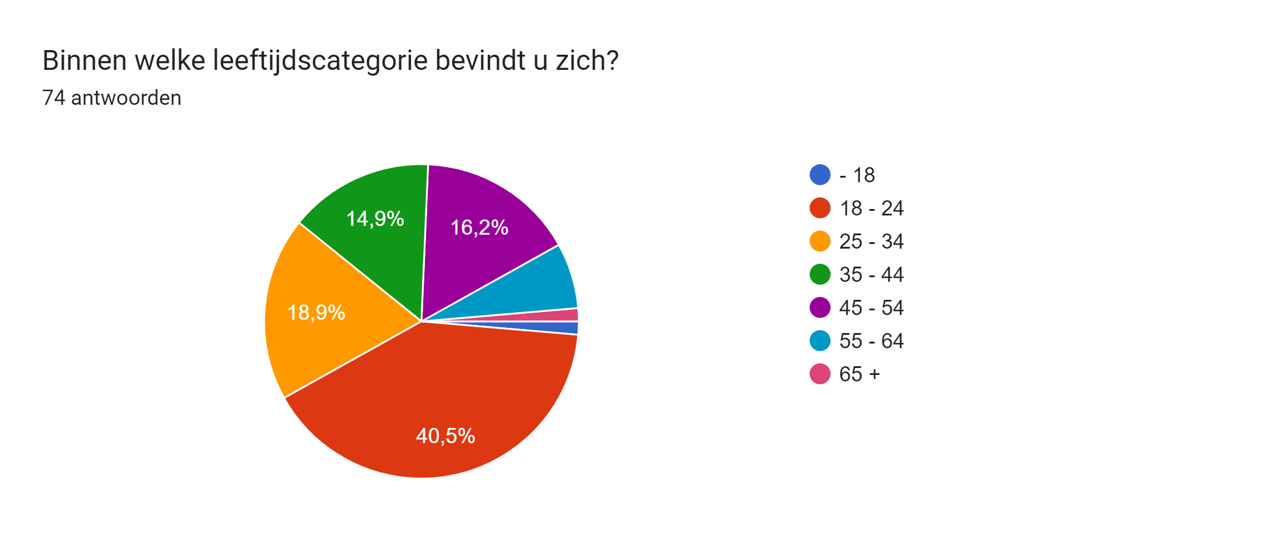
\includegraphics[width=0.9\textwidth]{i1.png}
    \label{fig:leeftijdsgroepen_resultaat}
\end{figure}

Van deze 74 personen gaf 44,6\% aan kennis van AI te hebben, en 55,4\% gaf aan geen kennis van AI te hebben.

\begin{figure}[htbp]
    \centering
    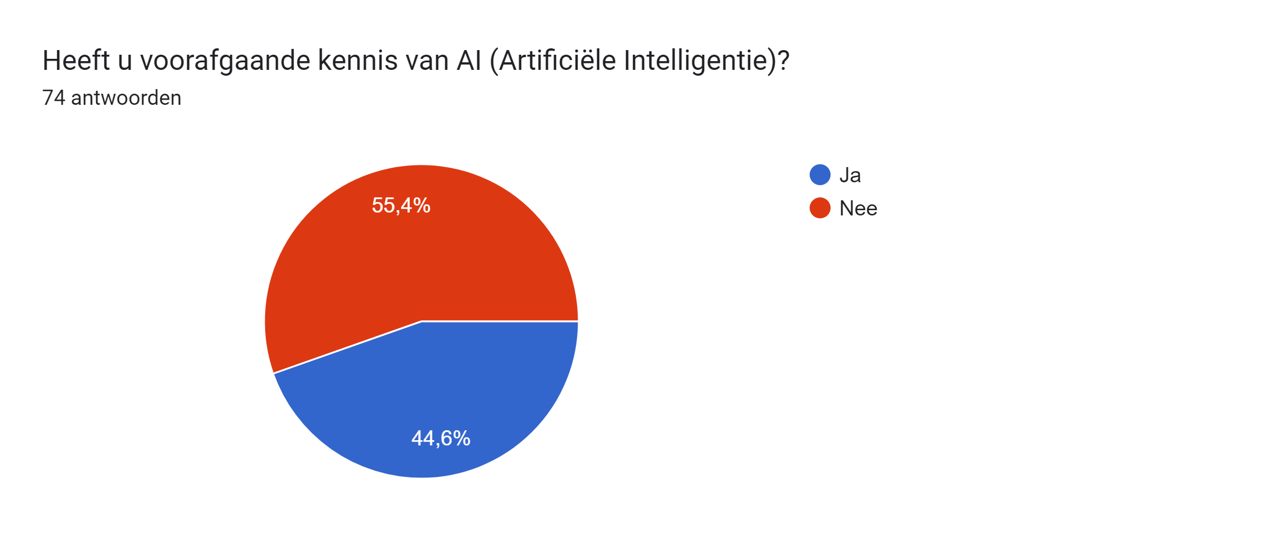
\includegraphics[width=0.9\textwidth]{i2.png}
    \label{fig:ai_kennis_resultaat}
\end{figure}

Hier onder volgt een overzicht van de vragen met bijgevolg een overzicht van de resultaten.

\subsubsection{De applicatie is in staat je te herkennen}

Dit wil zeggen dat de applicatie in staat is om uw identiteit vast te stellen. Dit betekent dat de applicatie kan detecteren wie er voor de camera zit tijdens een videogesprek. Op basis van deze herkenning kan de applicatie vervolgens gesprekken aanpassen en specifieke interacties mogelijk maken, afhankelijk van uw identiteit.

Dit aspect doelde op de gezichtsherkenning.

\begin{figure}[htbp]
    \centering
    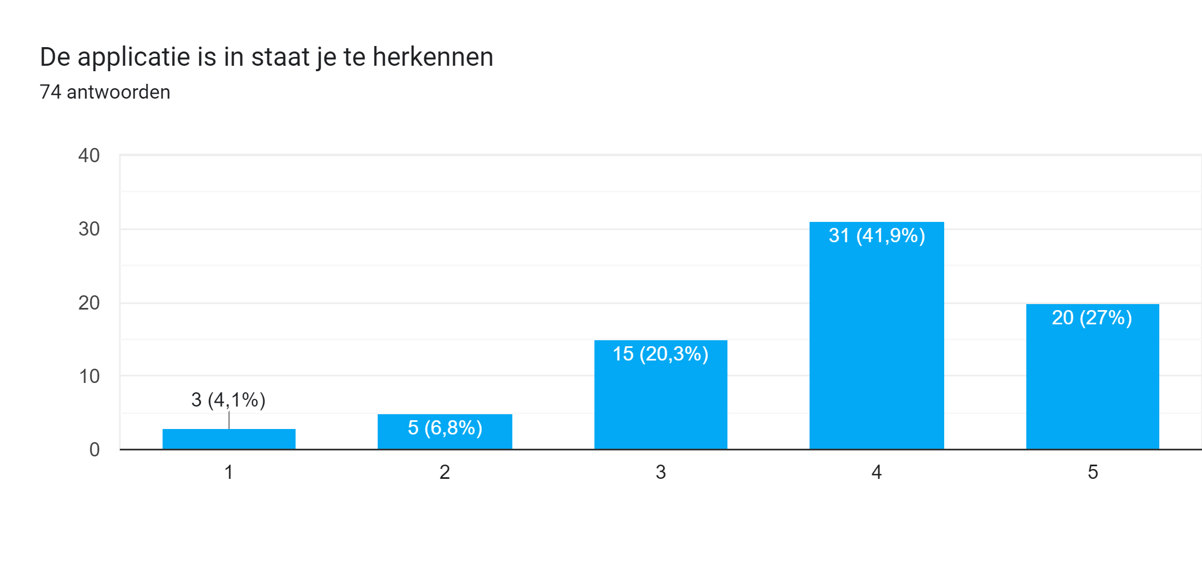
\includegraphics[width=0.9\textwidth]{q1.png}
    \label{fig:vraag_1_resultaat}
\end{figure}

\subsubsection{De applicatie is in staat emoties te herkennen}

Dit wil zeggen  dat de applicatie in staat is om emoties af te lezen aan uw gezichtsuitdrukkingen tijdens een videogesprek. Op basis van deze emotionele detectie kan de applicatie vervolgens gepaste reacties genereren die afgestemd zijn op uw emotionele toestand.

Dit aspect doelde op de emotieherkenning.

\begin{figure}[htbp]
    \centering
    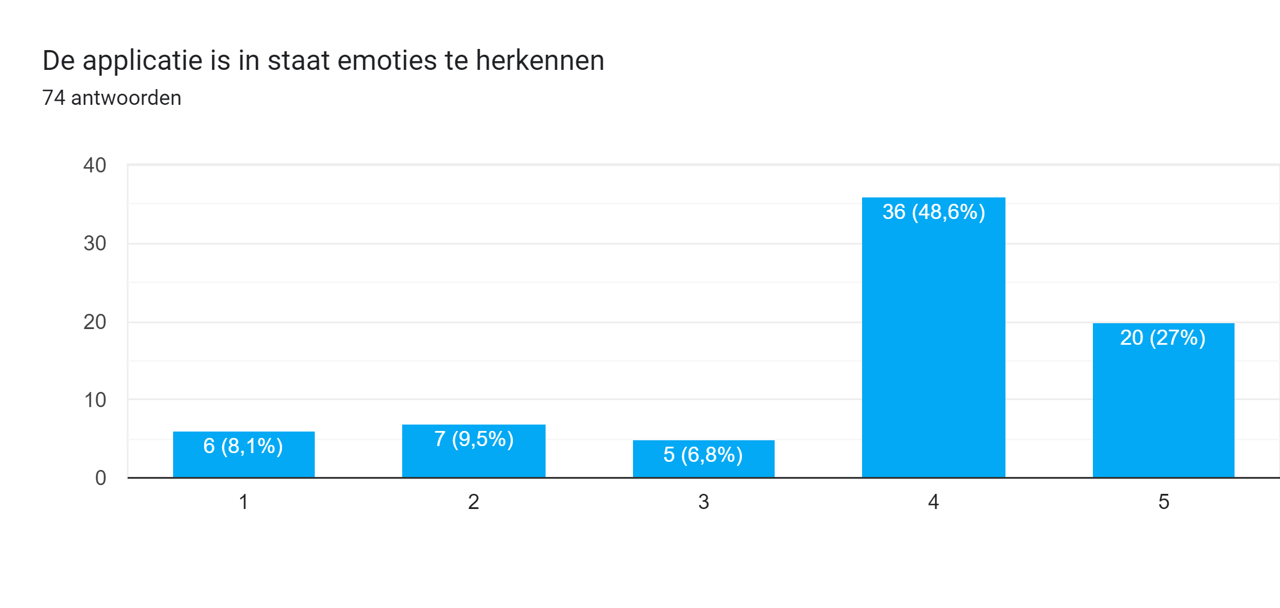
\includegraphics[width=0.9\textwidth]{q2.png}
    \label{fig:vraag_2_resultaat}
\end{figure}

\subsubsection{De persoon (tegenpartij) ziet er realistisch uit qua uiterlijk}

Dit wil zeggen dat de weergave van de persoon in de applicatie een hoge mate van menselijkheid heeft en bijna niet te onderscheiden is van een echt persoon. Dit houdt in dat de visuele weergave van de persoon zo nauwkeurig en gedetailleerd is dat het de illusie wekt van een werkelijk persoon in plaats van een geanimeerd of kunstmatig wezen.

Dit aspect doelde op de deepfakes.

\begin{figure}[htbp]
    \centering
    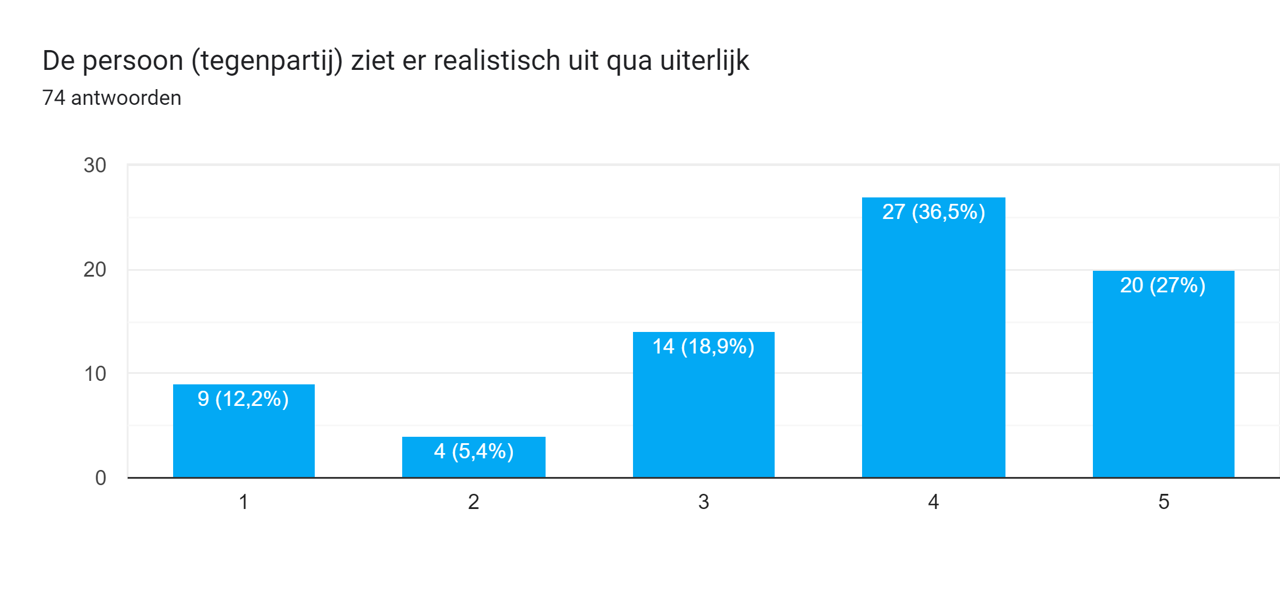
\includegraphics[width=0.9\textwidth]{q3.png}
    \label{fig:vraag_3_resultaat}
\end{figure}

\subsubsection{De applicatie verstaat zonder problemen wat u zegt}

Dit wil zeggen dat de applicatie in staat is om alles wat u zegt te begrijpen en correct te interpreteren. Dit houdt in dat de applicatie uw spraak nauwkeurig kan herkennen, taal kan begrijpen en correcte betekenis kan geven aan uw woorden en zinnen.

Dit aspect doelde op spraakherkenning en spraakverwerking.

\begin{figure}[htbp]
    \centering
    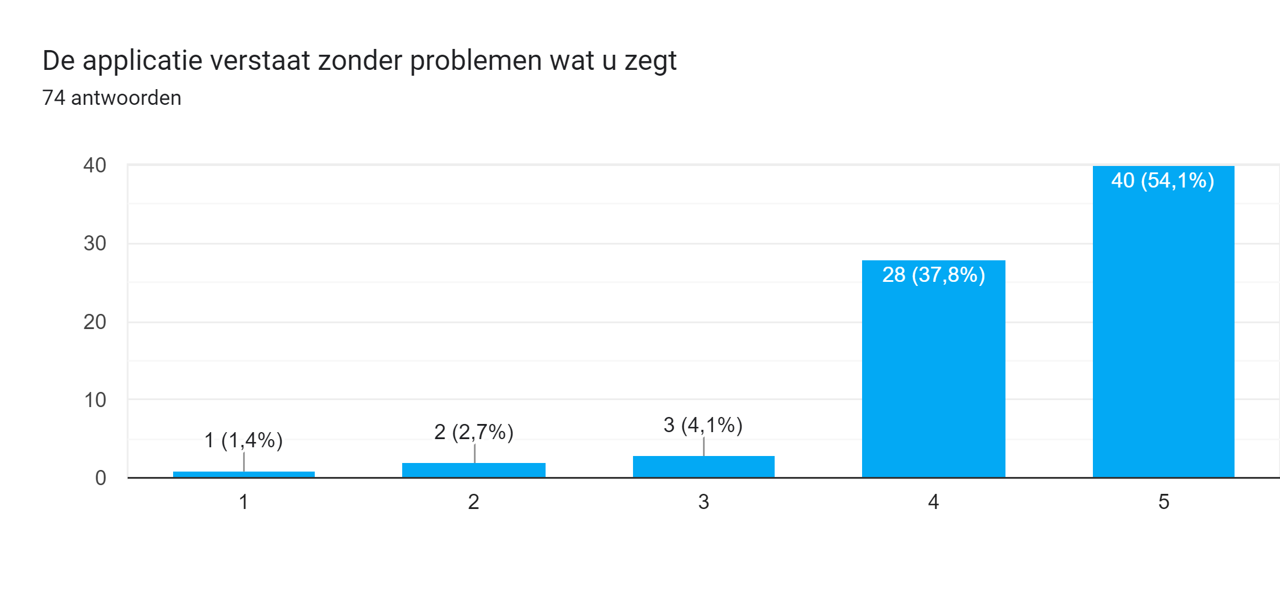
\includegraphics[width=0.9\textwidth]{q4.png}
    \label{fig:vraag_4_resultaat}
\end{figure}

\subsubsection{De applicatie kan zonder problemen antwoorden op wat u zegt}

Dit wil zeggen  dat de applicatie in staat is om goed geformuleerde en correcte antwoorden te geven op uw input. Dit houdt in dat de applicatie begrijpt wat u zegt en in staat is om relevante en zinvolle reacties te genereren. 

Dit aspect doelde op taalherkenning en taalverwerking.

\begin{figure}[htbp]
    \centering
    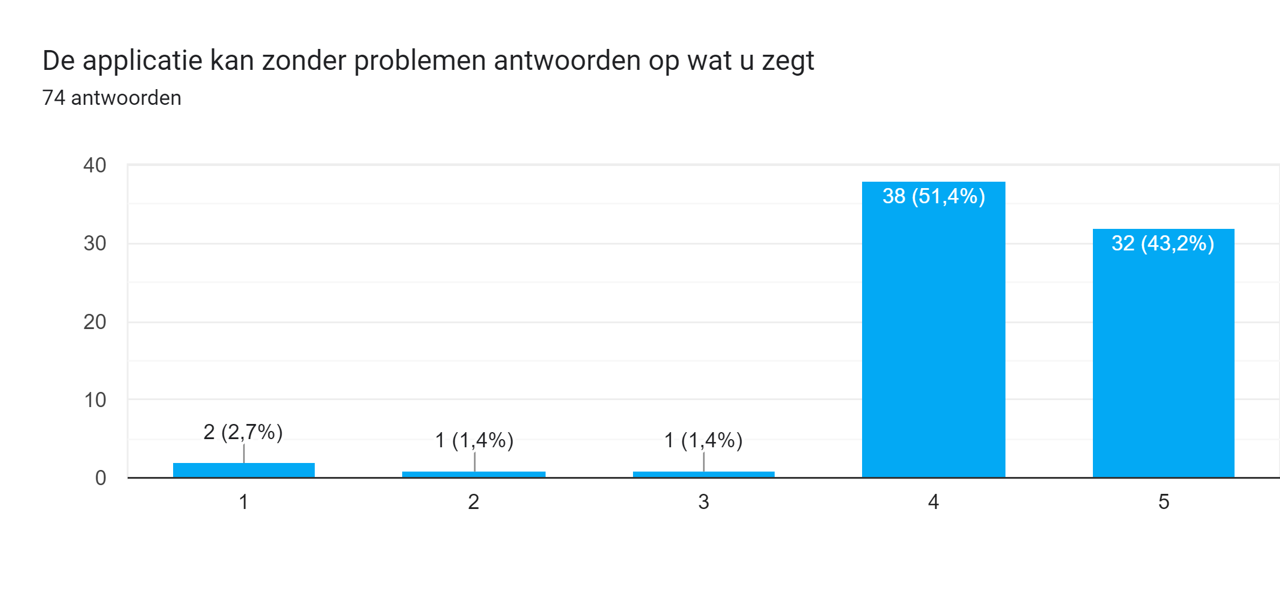
\includegraphics[width=0.9\textwidth]{q5.png}
    \label{fig:vraag_5_resultaat}
\end{figure}

\subsubsection{De stem van de applicatie klinkt zoals een menselijke stem}

Dit wil zeggen dat de stem die u hoort tijdens interactie met de applicatie niet te onderscheiden is van een stem van een echt persoon. Dit houdt in dat de stem natuurlijk, vloeiend en menselijk klinkt, waardoor het lijkt alsof u met een werkelijk persoon communiceert.

Dit aspect doelde op synthetische stemtechnologie.

\begin{figure}[htbp]
    \centering
    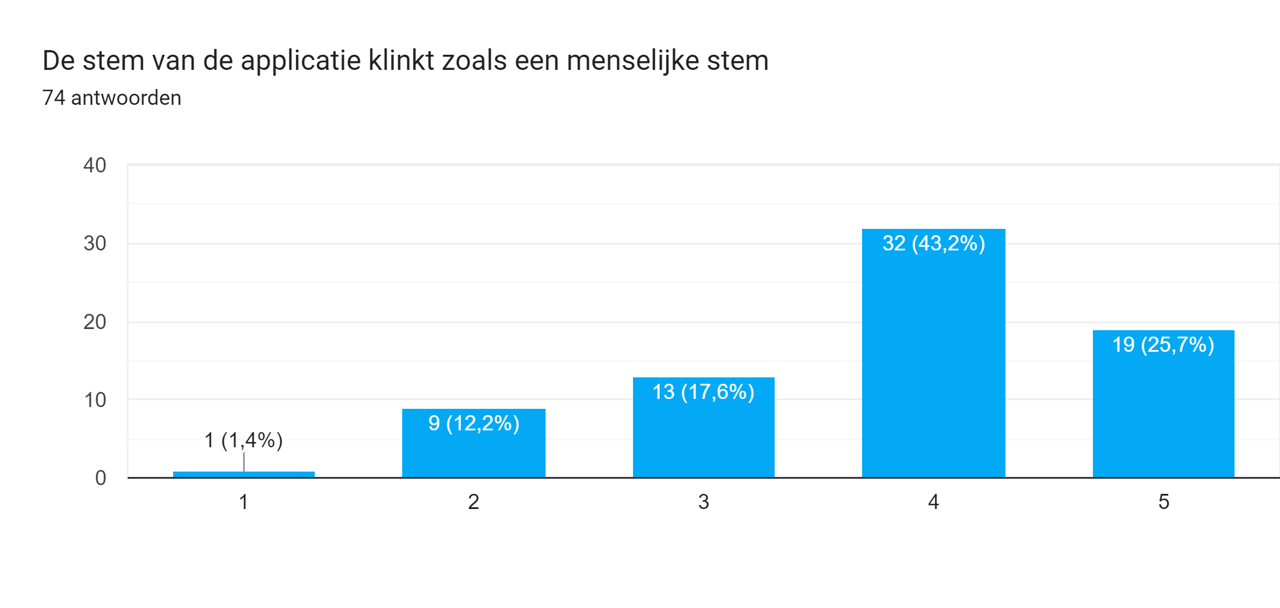
\includegraphics[width=0.9\textwidth]{q6.png}
    \label{fig:vraag_6_resultaat}
\end{figure}

\subsubsection{De applicatie heeft algemene kennis \& skills en kan deze ook aanleren}

Dit wil zeggen dat de applicatie beschikt over een brede basis van algemene kennis en vaardigheden. U kunt de applicatie vragen stellen die worden beschouwd als algemene kennis, zoals recente gebeurtenissen in de wereld. Bovendien is de applicatie ook in staat om nieuwe informatie en vaardigheden aan te leren naarmate u met de applicatie interacties heeft.

Dit aspect doelde op algemene kennis en skills verwerven en verbeteren.

\begin{figure}[htbp]
    \centering
    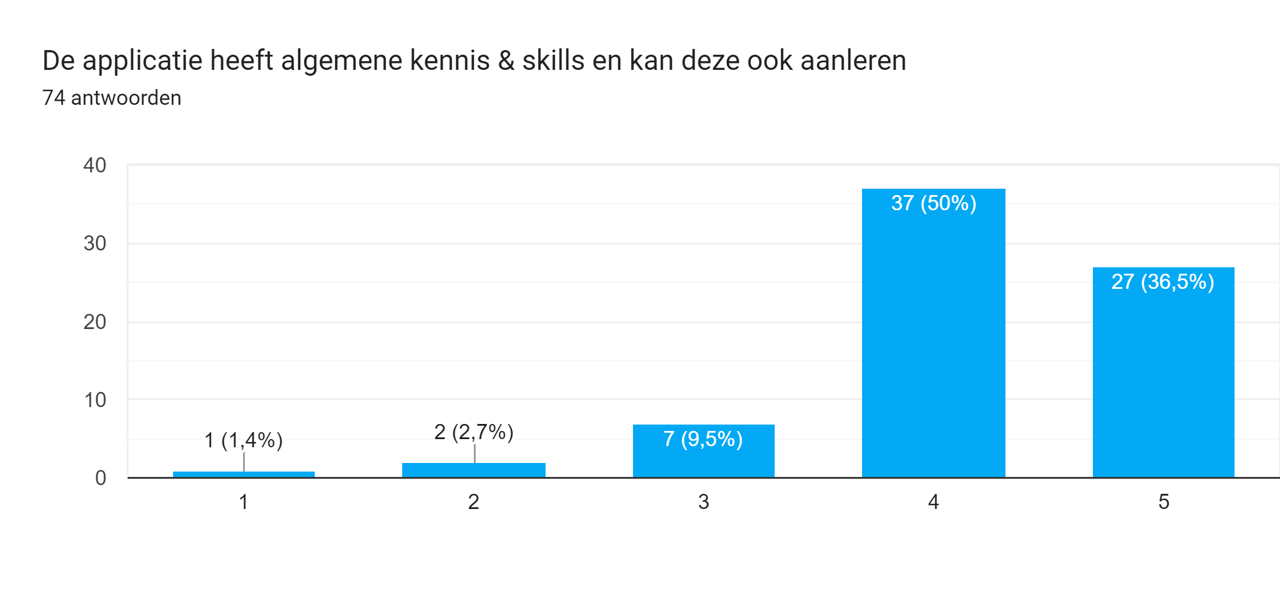
\includegraphics[width=0.9\textwidth]{q7.png}
    \label{fig:vraag_7_resultaat}
\end{figure}

\subsubsection{De applicatie begrijpt persoonlijkheden}

Dit wil zeggen dat de applicatie in staat is om verschillende persoonlijkheden te herkennen en te begrijpen. Hierdoor kan de applicatie een gepersonaliseerde interactie bieden die aansluit bij uw voorkeuren en behoeften. Dit houdt in dat de applicatie kan inspelen op uw persoonlijkheid en een aangepaste respons kan geven die bij uw stijl en voorkeuren past.

Dit aspect doelde op persoonlijkheidsmodellering.

\begin{figure}[htbp]
    \centering
    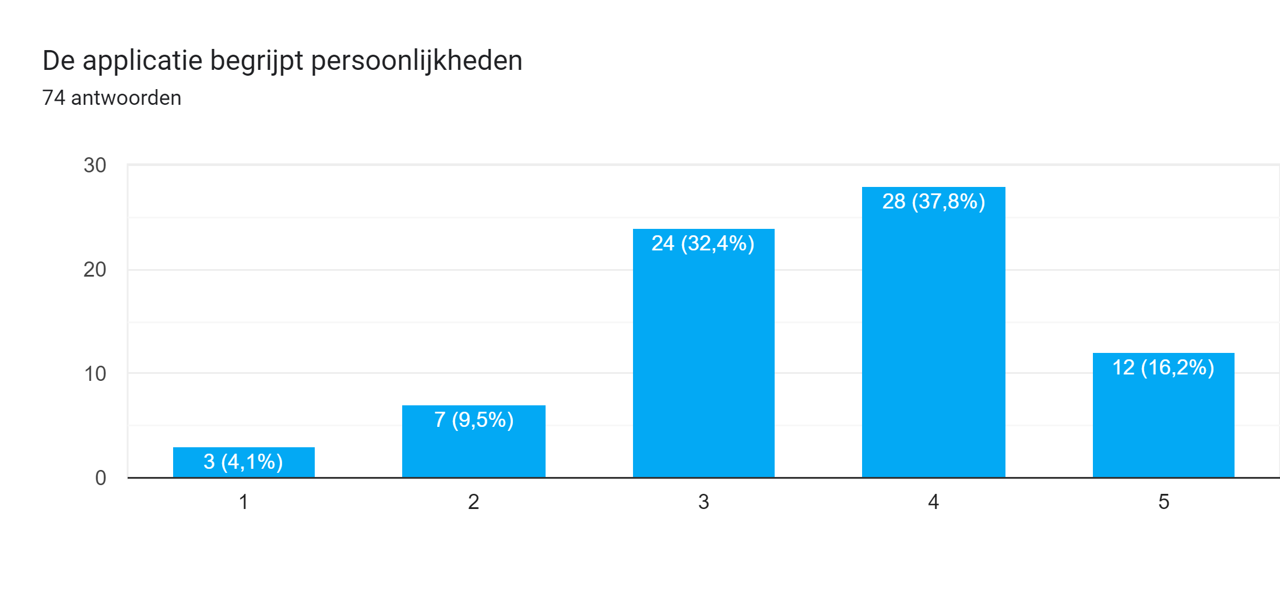
\includegraphics[width=0.9\textwidth]{q8.png}
    \label{fig:vraag_8_resultaat}
\end{figure}

\subsubsection{De applicatie begrijpt context}

Dit wil zeggen dat de applicatie in staat is om de context te begrijpen door zowel de spraak als het beeld van de tegenpartij te analyseren. Dit zorgt ervoor dat de applicatie bij het geven van antwoorden rekening houdt met de context en in staat is om de intentie achter de gestelde vraag te achterhalen. Hierdoor kan de applicatie beter passende antwoorden geven die aansluiten bij de context en de behoeften van de gebruiker.

Dit aspect doelde op contextueel begrip.

\begin{figure}[htbp]
    \centering
    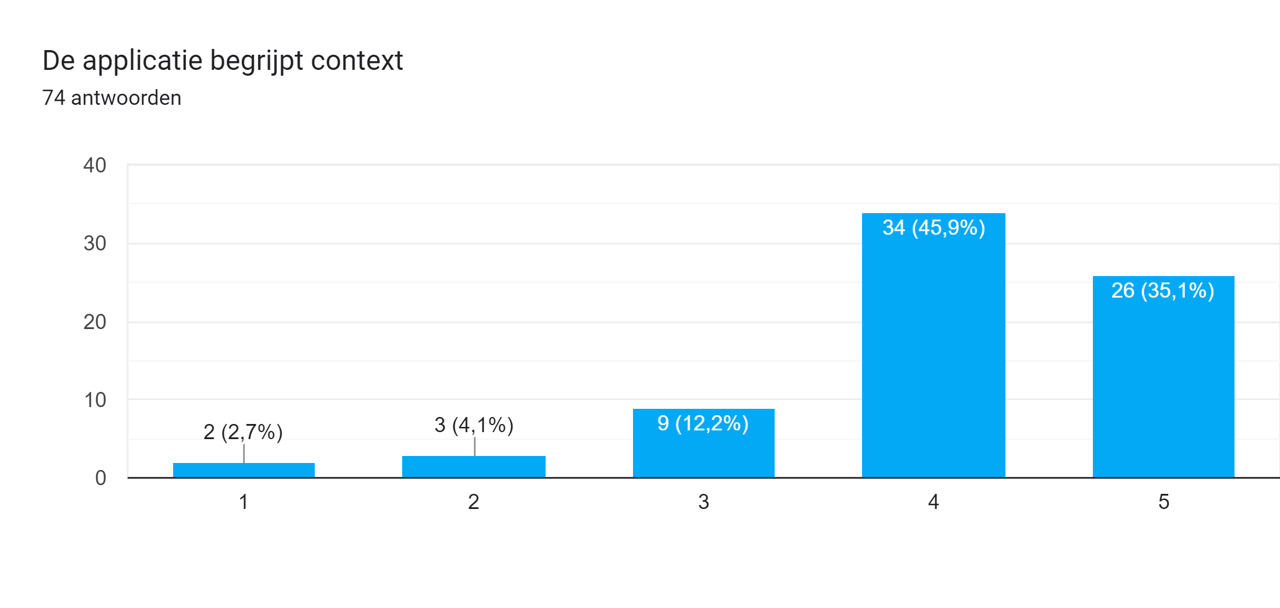
\includegraphics[width=0.9\textwidth]{q9.png}
    \label{fig:vraag_9_resultaat}
\end{figure}